\documentclass{standalone}
\usepackage{tikz}
\usetikzlibrary{patterns}
\usetikzlibrary{positioning}
\usetikzlibrary{patterns, positioning}
\usetikzlibrary{shapes.misc}
\usepackage[outline]{contour}
\contourlength{1.5pt} 
\usepackage[sfdefault]{ClearSans}

\begin{document}
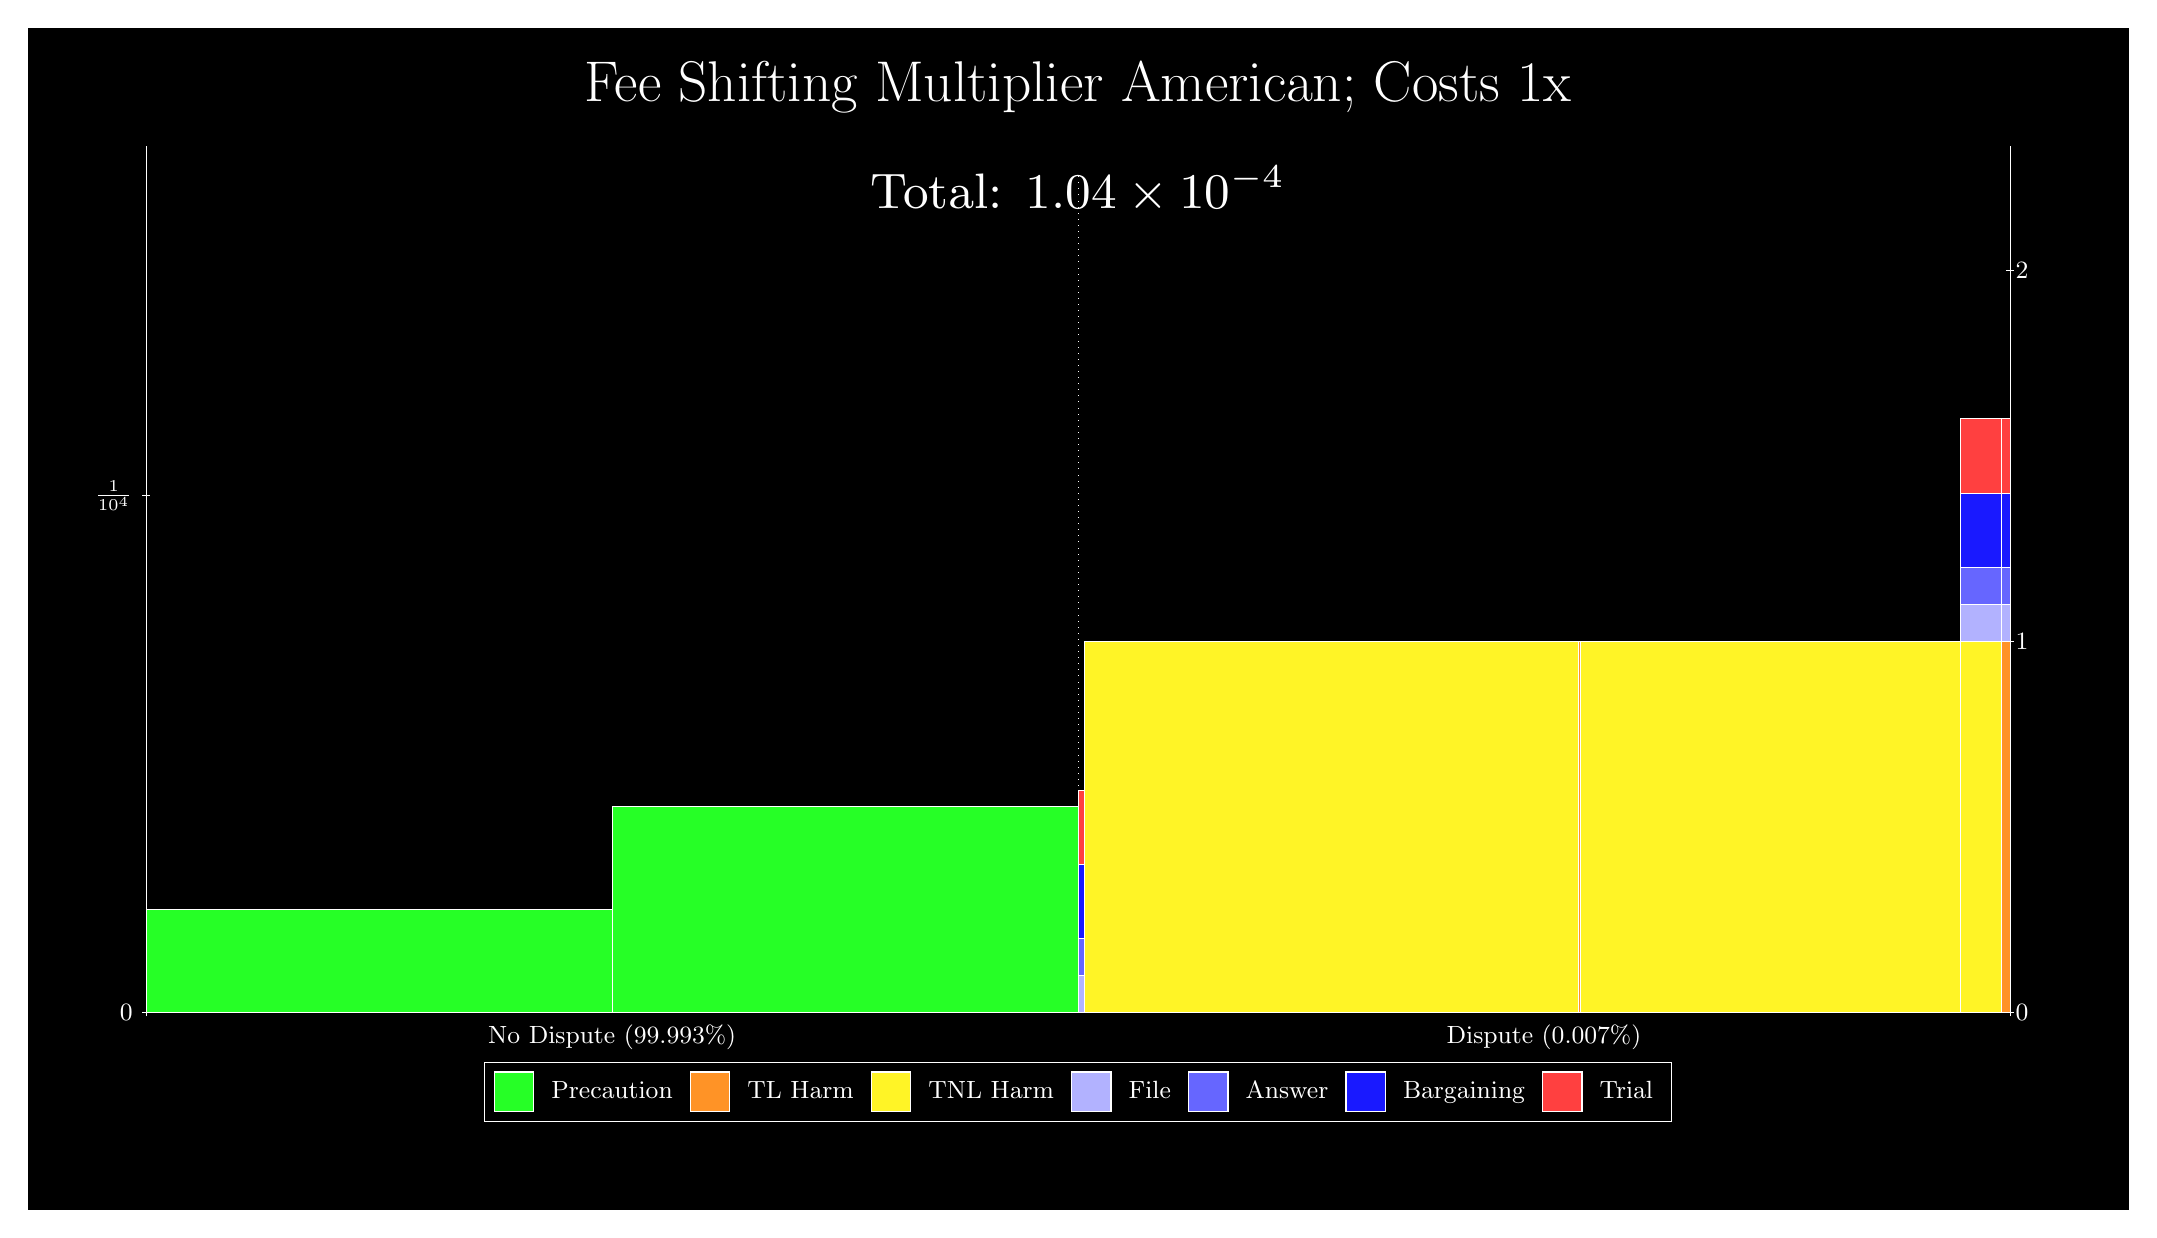
\begin{tikzpicture}
\draw[fill=black] (0,0) rectangle (26.667,15);
\draw[draw=none,text=white] (0,13.5) rectangle (26.667,15) node[midway] {\huge Fee Shifting Multiplier American; Costs 1x};
\draw[fill=green!85,draw=white,very thin] (1.5,2.5) rectangle (7.4166,3.8124);
\draw[fill=green!85,draw=white,very thin] (7.4166,2.5) rectangle (13.333,5.1248);
\draw[fill=green!85,draw=white,very thin] (13.333,2.5) rectangle (13.413,2.5001);
\draw[fill=blue!30,draw=white,very thin] (13.333,2.5001) rectangle (13.413,2.9714);
\draw[fill=blue!60,draw=white,very thin] (13.333,2.9714) rectangle (13.413,3.4428);
\draw[fill=blue!90,draw=white,very thin] (13.333,3.4428) rectangle (13.413,4.3854);
\draw[fill=red!75,draw=white,very thin] (13.333,4.3854) rectangle (13.413,5.3281);
\draw[fill=green!85,draw=white,very thin] (13.413,2.5) rectangle (19.686,2.5001);
\draw[fill=yellow!85,draw=white,very thin] (13.413,2.5001) rectangle (19.686,7.2134);
\draw[fill=green!85,draw=white,very thin] (19.686,2.5) rectangle (19.717,2.5001);
\draw[fill=orange!85,draw=white,very thin] (19.686,2.5001) rectangle (19.717,7.2134);
\draw[fill=green!85,draw=white,very thin] (19.717,2.5) rectangle (24.541,2.5002);
\draw[fill=yellow!85,draw=white,very thin] (19.717,2.5002) rectangle (24.541,7.2135);
\draw[fill=green!85,draw=white,very thin] (24.541,2.5) rectangle (25.061,2.5001);
\draw[fill=yellow!85,draw=white,very thin] (24.541,2.5001) rectangle (25.061,7.2134);
\draw[fill=blue!30,draw=white,very thin] (24.541,7.2134) rectangle (25.061,7.6848);
\draw[fill=blue!60,draw=white,very thin] (24.541,7.6848) rectangle (25.061,8.1561);
\draw[fill=blue!90,draw=white,very thin] (24.541,8.1561) rectangle (25.061,9.0988);
\draw[fill=red!75,draw=white,very thin] (24.541,9.0988) rectangle (25.061,10.041);
\draw[fill=green!85,draw=white,very thin] (25.061,2.5) rectangle (25.167,2.5001);
\draw[fill=orange!85,draw=white,very thin] (25.061,2.5001) rectangle (25.167,7.2134);
\draw[fill=blue!30,draw=white,very thin] (25.061,7.2134) rectangle (25.167,7.6848);
\draw[fill=blue!60,draw=white,very thin] (25.061,7.6848) rectangle (25.167,8.1561);
\draw[fill=blue!90,draw=white,very thin] (25.061,8.1561) rectangle (25.167,9.0988);
\draw[fill=red!75,draw=white,very thin] (25.061,9.0988) rectangle (25.167,10.041);
\node[font=\small,text=white,anchor=north,scale=2] at (13.333, 13.5) {Total: $1.04\times 10^{-4}$};
\draw[white,very thin] (1.5,2.5) -- (1.5,13.5);
\draw[white,very thin] (1.45,2.5) -- (1.55,2.5);
\node[font=\small,text=white, anchor=east] at (1.45, 2.5) {0};
\draw[white,very thin] (1.45,9.062) -- (1.55,9.062);
\node[font=\small,text=white, anchor=east] at (1.45, 9.062) {$\frac{1}{10^{4}}$};

\draw[white,dotted,very thin] (13.333,2.83) -- (13.333,13.17);
\draw[white,very thin] (25.167,2.5) -- (25.167,13.5);
\draw[white,very thin] (25.117,2.5) -- (25.217,2.5);
\node[font=\small,text=white, anchor=west] at (25.117, 2.5) {0};
\draw[white,very thin] (25.117,7.2134) -- (25.217,7.2134);
\node[font=\small,text=white, anchor=west] at (25.117, 7.2134) {1};
\draw[white,very thin] (25.117,11.927) -- (25.217,11.927);
\node[font=\small,text=white, anchor=west] at (25.117, 11.927) {2};

\draw[white,very thin] (1.5,2.5) -- (25.167,2.5);
\draw[white,very thin] (1.5,2.45) -- (1.5,2.55);
\node[font=\small,text=white, anchor=north] at (1.5, 2.45) {};
\draw[white,very thin] (25.167,2.45) -- (25.167,2.55);
\node[font=\small,text=white, anchor=north] at (25.167, 2.45) {};

\node[font=\small,text=white,anchor=south] at (7.4167, 1.9) {No\ Dispute\ (99.993\%)};
\node[font=\small,text=white,anchor=south] at (19.25, 1.9) {Dispute\ (0.007\%)};
\draw (13.3333,2.5) node (B) {};
\begin{scope}[align=center]
\matrix[scale=0.5,draw=white,below=0.5cm of B,nodes={draw},column sep=0.1cm]{
\node[rectangle,draw,minimum width=0.5cm,minimum height=0.5cm,fill=green!85]{}; & \node[draw=none,font=\small,text=white]{Precaution}; &
\node[rectangle,draw,minimum width=0.5cm,minimum height=0.5cm,fill=orange!85]{}; & \node[draw=none,font=\small,text=white]{TL Harm}; &
\node[rectangle,draw,minimum width=0.5cm,minimum height=0.5cm,fill=yellow!85]{}; & \node[draw=none,font=\small,text=white]{TNL Harm}; &
\node[rectangle,draw,minimum width=0.5cm,minimum height=0.5cm,fill=blue!30]{}; & \node[draw=none,font=\small,text=white]{File}; &
\node[rectangle,draw,minimum width=0.5cm,minimum height=0.5cm,fill=blue!60]{}; & \node[draw=none,font=\small,text=white]{Answer}; &
\node[rectangle,draw,minimum width=0.5cm,minimum height=0.5cm,fill=blue!90]{}; & \node[draw=none,font=\small,text=white]{Bargaining}; &
\node[rectangle,draw,minimum width=0.5cm,minimum height=0.5cm,fill=red!75]{}; & \node[draw=none,font=\small,text=white]{Trial}; \\\\
};\end{scope}

\end{tikzpicture}
\end{document}